\documentclass[border=3pt]{standalone}
% Shared preamble for every generated figure.
% Matches the report: newtx (Times), greyscale, square boxes.
\usepackage{newtxtext,newtxmath}
% newtx's typewriter (txtt) draws a slashed zero; use Latin Modern instead.
\renewcommand{\ttdefault}{lmtt}
\usepackage{tikz}
\usetikzlibrary{positioning,arrows.meta,calc,fit,backgrounds,shapes.geometric,
                decorations.pathreplacing,decorations.pathmorphing,matrix,patterns}

\definecolor{figgrey}{gray}{0.88}
\definecolor{figmid}{gray}{0.60}
\definecolor{figdark}{gray}{0.35}

\tikzset{
  fig/.style={font=\small},
  box/.style={draw,thick,minimum height=8mm,minimum width=22mm,align=center,
              inner sep=2pt,font=\small},
  greybox/.style={box,fill=figgrey},
  smallbox/.style={draw,minimum height=6mm,minimum width=16mm,align=center,
                   inner sep=2pt,font=\scriptsize},
  ln/.style={-{Stealth[length=2.2mm,width=1.8mm]},thick},
  lnb/.style={{Stealth[length=2.2mm,width=1.8mm]}-{Stealth[length=2.2mm,width=1.8mm]},thick},
  lbl/.style={font=\scriptsize,inner sep=1.5pt},
  note/.style={font=\scriptsize\itshape,inner sep=1.5pt},
}

\begin{document}
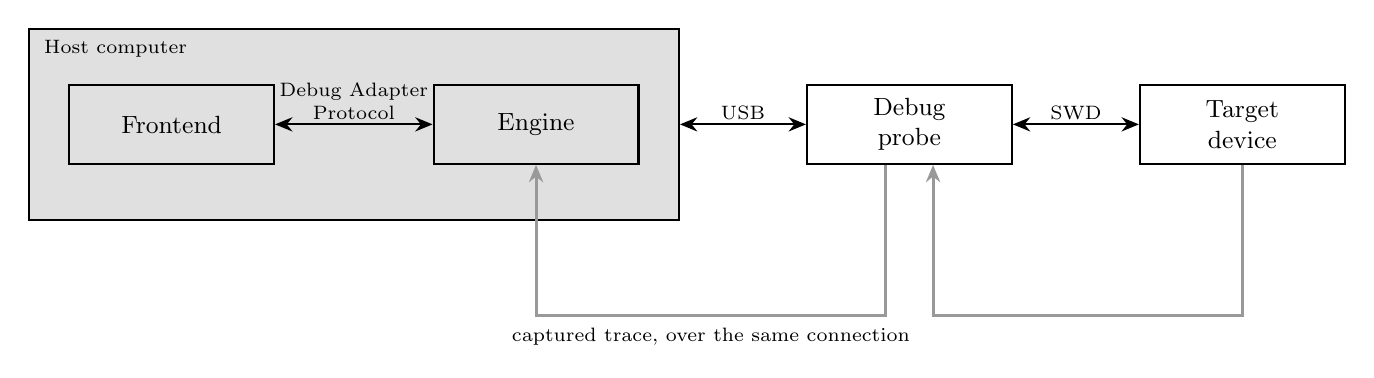
\begin{tikzpicture}[fig,
  el/.style={draw,thick,minimum height=10mm,minimum width=26mm,align=center,font=\small},
  tr/.style={-{Stealth[length=2.2mm,width=1.8mm]},thick,figmid,line width=1.1pt}]

\node[el] (en) {Engine};

\node[el,left=20mm of en] (fe) {Frontend};
\draw[lnb] (fe) -- node[lbl,above,align=center]{Debug Adapter\\Protocol} (en);

\begin{scope}[on background layer]
  \node[draw,thick,fill=figgrey,fit=(fe)(en),inner xsep=5mm,inner ysep=7mm] (host) {};
\end{scope}
\node[lbl,anchor=north west] at ($(host.north west)+(1.5mm,-1mm)$) {Host computer};

\node[el,right=16mm of host] (pr) {Debug\\probe};
\node[el,right=16mm of pr] (tg) {Target\\device};

\draw[lnb] (host.east) -- node[lbl,above]{USB} (pr.west);
\draw[lnb] (pr) -- node[lbl,above]{SWD} (tg);

\coordinate (ry) at ($(host.south)+(0,-12mm)$);
\coordinate (ee) at (en.south);
\coordinate (pl) at ($(pr.south)+(-3mm,0)$);
\coordinate (prr) at ($(pr.south)+(3mm,0)$);
\draw[tr] (tg.south) -- (tg.south |- ry) -- (prr |- ry) -- (prr);
\draw[tr] (pl) -- (pl |- ry) -- (ee |- ry) -- (ee);
\node[lbl,below=1mm] at ($(pl |- ry)!0.5!(ee |- ry)$) {captured trace, over the same connection};

\end{tikzpicture}
\end{document}
